\documentclass[a4paper]{article}

%% Language and font encodings
\usepackage[english]{babel}
\usepackage[utf8]{inputenc}
\usepackage{tabu}
\usepackage[T1]{fontenc}
\usepackage{enumitem}
\usepackage{amsmath}
\usepackage{xcolor}
\usepackage{amsfonts}

%% Sets page size and margins
\usepackage[a4paper,top=3cm,bottom=2cm,left=3cm,right=3cm,marginparwidth=1.75cm]{geometry}

%% Useful packages
\usepackage{amsmath}
\usepackage{graphicx}
\usepackage{fancyhdr}
\usepackage{makecell}

\renewcommand\theadalign{bc}
\renewcommand\theadfont{\bfseries}
\renewcommand\theadgape{\Gape[4pt]}
\renewcommand\cellgape{\Gape[4pt]}
%% Title
\title{\textbf{Playing card detection}\\ PlayCDC\\Object recognition and image understanding lecture}
\author{Frank Gabel and Daniel Gonzalez}

\date{15.07.2018}

\begin{document}
\maketitle
\section{Abstract}
With the capabilities of upcoming small video capturing devices in, for example, smart contact lenses with built-in cameras, whole new ways of cheating in cardgames emerge. In order to help facilitate these cheating endeavours, we implement an algorithm that detects the suits and ranks of playing cards in the field of view of a camera using the latest iteration of the YOLO object recognition algorithm.
\begin{figure}[h]
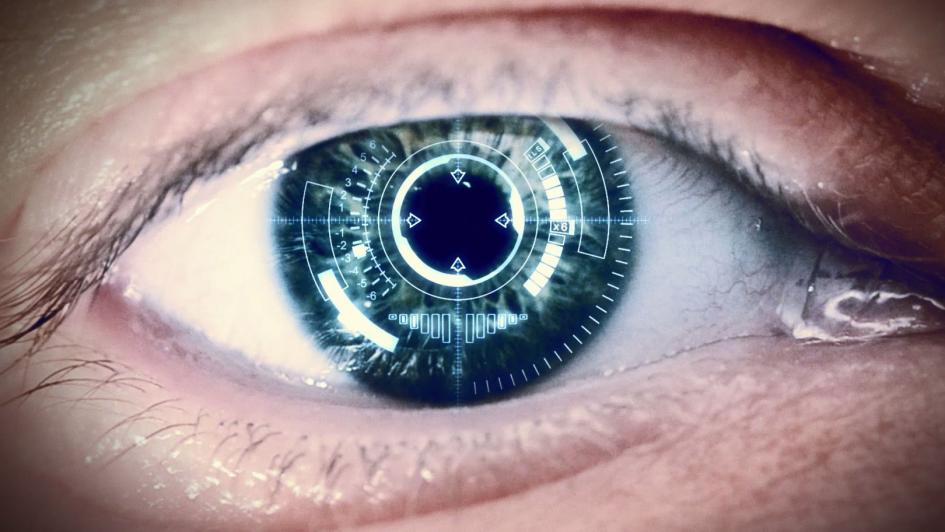
\includegraphics[scale=0.25]{contact_lense}
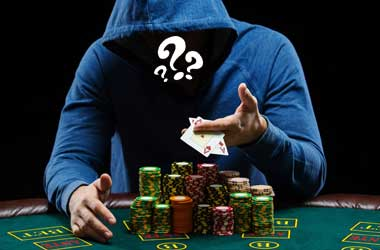
\includegraphics[scale=0.532]{poker_player}
\caption{Stock photos of an envisioned camera-equipped contact lense (left) and a mysterious black-jack player (right)}
\end{figure}
\section{Introduction}
A big topic in computer vision is the search of methods that are, given a query image, capable of answering questions like: What is present in an image? Is there a particular object in it? Where exactly in the image is this object located? Is it possible to semantically segment objects of interest in the image?
Object detection deals with detecting instances of semantic objects of a certain class (such as humans, buildings, or cars) in digital images and videos. Typically, object detection deals with two sub-taks: \textbf{object localization} using bounding boxes and \textbf{multiclass object classification} within said bounding boxes.
Sometimes, a third sub-task of \textbf{semantic object segmentation} is performed, i.e. the process of labelling objects on pixel level.\\
In this project, we use the YOLOv3 object detection algorithm (CITE) for object detection (without additional segmentation) in order to tell apart playing cards of a standard 52-part deck.

\section{Dataset}
DANIEL THAT'S YOUR PLAYGROUND, PLEASE PUT A COUPLE OF PHOTOS :)))
As there was no suitable dataset of cards to use, we decided to create it by our own.  We did this in basically three main steps to obtain at the end \textbf{(Nr. images)}images,  as well as the necessary  Bounding Box information required for training our YOLO NN.   First we had to create the data doing photos and arrange it in such a way that  we can easily use it around our workflow.  The next, we had to detect the convex hulls of the card numbers and suits and the last perform rotations/re scaling/... on the images to generate new data.\\ \\
\subsection{dataset synthesis pipeline}


\large \textbf{Data preparation} \\
\normalsize
We decided to work with a deck of 52 cards, where each card contain two times the card logo.  We took for each card 2 different photos \textbf{(TODO: check this there were not really 52)} and after this we extract the cards of the photos and re-scaled them to 600x900 pixels.  We choose this resolution arbitrary, as we though that it was a nice size to work with.
For this part, we used the selection/rotation/cropping/re-scale -tools provided by GIMP\footnote{GIMP 2.8.22 - GNU Image Manipulation Program}.
Concluding this, we proceed by detecting the convex hulls of the cards numbers and suits.  We detect the convex hulls using SciPy libraries\footnote{SciPy: Open Source Scientific Tools for Python}in a semi-automatic way, verifying for each card manually that we got the desired result \textbf{[SEE FIGURE]}.
At the last step, we saved the convex hulls as an NumPy array \textbf{(cite??)} \\ \\
\large \textbf{Data generation} \\
\normalsize
The goal in this step was to generate a big amount of new data for each card destined for training or NN. We wanted to perform image transformations, like translations, rotations and re scaling, as well as blurring and sharping to generate new data.  We decided to use the imgaug python library, because it provided a nice way to keep track of the convex hulls after doing transformations. 
\section{Related work - The object detection landscape}
The task of object detection in images encompasses both the "simple" form of localizing and subsequently classifying objects as well as the more "advanced" form of additionally segmenting objects pixel-wise. For these task, different deep learning architectures have emerged, of which we will present the most important ones in the following.\\ In 2015, \textbf{Faster Region-based Convolutional Network (Faster R-CNN)} (CITE) has come up as an enhancement of the existing R-CNN and Fast R-CNN methods that are based on both region proposal networks to find candidate bounding boxes and detection networks to perform classification. Faster R-CNN extend this by introducing weight sharing  of the convolutional features between region proposal network and detection network, facilitating nearly cost-free region proposals. 

\textbf{You Only Look Once (YOLO)}
\textbf{Single-Shot Detector (SSD)}

\textbf{Focal Loss for Dense Object Detection (RetinaNet)}
\textbf{Mask Region-based Convolutional Network (Mask R-CNN)}
The Mask-RCNN consitutes the current state-of-the-art in semantic object segmentation. The basic idea is to.....
As this extends the scope of our project, we will not dive deeper and rather refer interested readers to the orginal research paper (CITE) or ...
\section{Methods}
\subsection*{The YOLO approach to object detection}
The YOLO model’s novel motivation is that it re-frames
object detection as a single regression problem, directly
from image pixels to bounding box coordinates and class
probabilities. This means that the YOLO model only ”looks
once” at an image for object detection.
It works by dividing an image into $S\times S$ grid. Each grid
cell predicts $B$ bounding boxes and a confidence score for
each box. The confidence scores show how confident the
model is that there is an object in that bounding box. This
is formally defined as:

YOLO is implemented as a 32 layer deep convolutional
neural network (DNN). The open source implementation released
along with the paper is built upon a custom DNN
framework written by YOLO’s authors, called darknet 1
.
This application provides the baseline by which we compare
our implementation of YOLO 2
. Redmon et al. have
released several variants of YOLO. For our purposes, we
chose the variant "tiny YOLOv3" which is a simplified version of YOLOv3 for restricted environments such as ours.\footnote{https://github.com/pjreddie/darknet/blob/master/cfg/yolov3-tiny.cfg}. In places in which the paper lacks details, we refer to the baseline darknet implementation
to resolve ambiguities.
\subsubsection*{Loss function}
YOLO’s loss function must simultaneously solve the object detection and object classification tasks. This function
simultaneously penalizes incorrect object detections
as well as considers what the best possible classification
would be. We employ the stochastic gradient descent
optimization method offered by TensorFlow[10] with the
Adam optimizer [7] to minimize the cost function. We
implement the following loss function, composed of five
terms:
\begin{align*}
\lambda_\textbf{coord}
\sum_{i = 0}^{S^2}
    \sum_{j = 0}^{B}
     {\mathbb{1}}_{ij}^{\text{obj}}
            \left[
            \left(
                x_i - \hat{x}_i
            \right)^2 +
            \left(
                y_i - \hat{y}_i
            \right)^2
            \right]&\textbf{\ coordinate loss}
\\\\
+ \lambda_\textbf{coord} 
\sum_{i = 0}^{S^2}
    \sum_{j = 0}^{B}
         {\mathbb{1}}_{ij}^{\text{obj}}
         \left[
        \left(
            \sqrt{w_i} - \sqrt{\hat{w}_i}
        \right)^2 +
        \left(
            \sqrt{h_i} - \sqrt{\hat{h}_i}
        \right)^2
        \right]\\
+ \sum_{i = 0}^{S^2}
    \sum_{j = 0}^{B}
        {\mathbb{1}}_{ij}^{\text{obj}}
        \left(
            C_i - \hat{C}_i
        \right)^2&\textbf{\ objectness loss}
\\
+ \lambda_\textrm{noobj}
\sum_{i = 0}^{S^2}
    \sum_{j = 0}^{B}
    {\mathbb{1}}_{ij}^{\text{noobj}}
        \left(
            C_i - \hat{C}_i
        \right)^2\\ 
+ \sum_{i = 0}^{S^2}
{{1}}_i^{\text{obj}}
    \sum_{c \in \textrm{classes}}
        \left(
            p_i(c) - \hat{p}_i(c)
        \right)^2&\textbf{\ classification loss}
\end{align*}


\subsubsection*{techniques}
\begin{description}
\item[Non-max suppression] Non max suppression removes the low probability bounding boxes which are very close to a high probability bounding boxes.
\end{description}

\subsubsection*{tiny YOLO-v3}

The particular architecture we used for training on our dataset is \textbf{tiny YOLOv3} which essentially is a smaller version of YOLO for constrained environments.
\begin{figure}


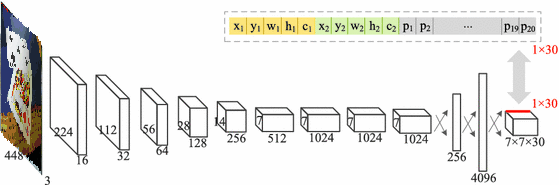
\includegraphics[width=1\linewidth]{tinyyolo}
\caption{tiny YOLO-v3 feature extractor}
\end{figure}

\subsection{Webcam deployment}
DANIEL
\subsection{Evaluation}
DANIEL - WRITE SOMETHING ABOUT MAP, YOU CAN PUT FORMULAS IN HERE LIKE A BOSS, BUILD UPON WHAT I WROTEIN THE POSTER MAYBE
\section{Results}
Our object detection endeavours using a tiny YOLOv3 detector resulted in diverse results depending on the complexity and pecularities of the synthesized dataset in use - the main results are summarize in REF TABLE 1 and REF FIGURE X. We generally achieved the best results for the datasets without textures and ....
In total, training always converged rather quickly. Again, datasets without complex textures led to better (i.e. faster) convergence which intuitively makes sense as the algorithm does not need to spend time ruling out complex dependencies that might be learned from unimportant pixels or regions outside the card.\\
\begin{table}[h]

\begin{tabular}{lllllr}
\hline
\multicolumn{5}{c}{Dataset situation} \\
\cline{1-2}
name    & description  & precision & recall & mAP \\
\hline
\textbf{1 - Simple}      & Paste cards on simple canvases    &  0.977  & 0.983 & \textbf{0.991} \\
          & \textit{random rotations, brightness, blurring}     &  & & \\
\textbf{2 - Medium}      & Paste randomly scaled cards on simple canvases & 0.977 & 0.983 & \textbf{0.991} \\
          & \textit{random rotations, brightness, blurring}     &  13 & & \\
\textbf{3 - Elaborate}       & Paste randomly scaled cards on textures & 0.977 & 0.983 & \textbf{0.991} \\
          & \textit{random rotations, brightness, blurring}     &  13 & & \\
\textbf{4 - Hardest} & Paste randomly scaled cards on textures & 0.977 & 0.983 & \textbf{0.991} \\
          & \textit{random rotations, brightness, blurring, more zoom}     &  13 & & \\
\hline


\end{tabular}
\caption{Your caption here} 
\end{table}
\subsection*{Exemplary test results and failure cases}
Metrics are helpful in measuring the effectiveness of algorithms, but computer vision often allows for an additional sensoric inspection of results using our human visual perceptive system. \\Hence, we compiled a couple of results on unseen test images (REF FIGURE3).
\begin{figure}[h]

\begin{tabular}{ccc}

 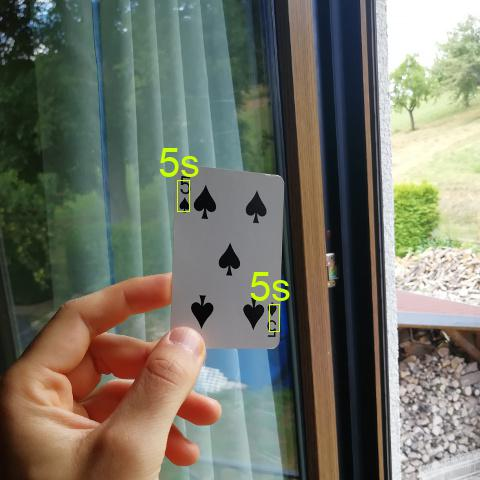
\includegraphics[width=44mm]{success3} &   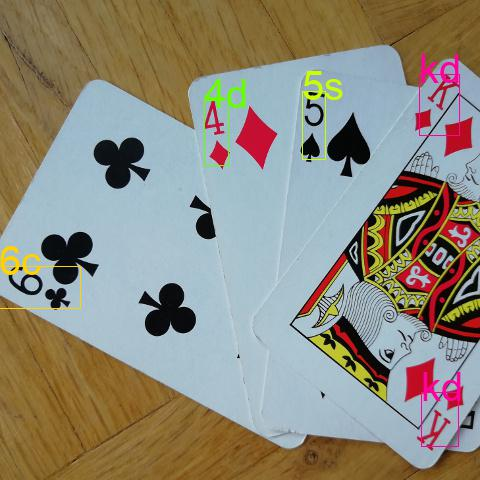
\includegraphics[width=44mm]{success2} &   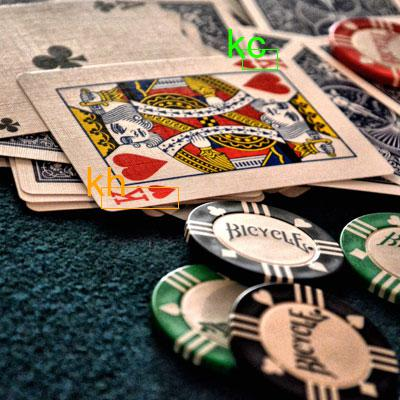
\includegraphics[width=44mm]{success1}\\
\makecell{\textbf{success:} scenario with a \\ highly diverse background}  & \makecell{\textbf{success:}  multiple cards \\ with trivial background} & \makecell{\textbf{success:}  angled shot of sheared card \\ in front of highly diverse background}\\[6pt]
  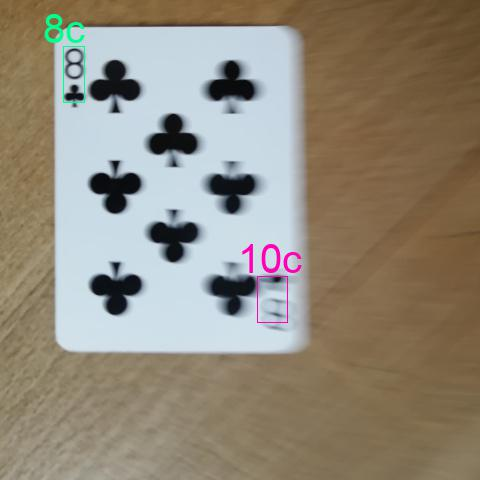
\includegraphics[width=44mm]{fail1} &   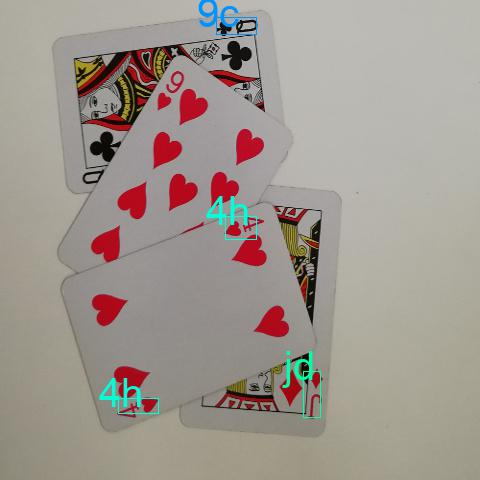
\includegraphics[width=44mm]{fail2} &   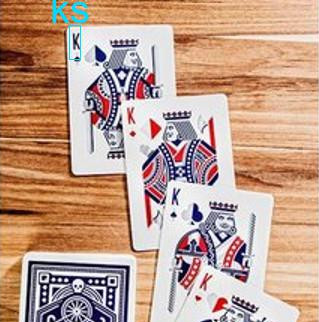
\includegraphics[width=44mm]{fail3}\\
\makecell{\textbf{fail:}  misdetection of 8c \\ due to motion blur} & \makecell{\textbf{fail:} misdetection of Qc and non- \\detection of 9h for unknown reason} & \makecell{\textbf{fail:} non-detection of Kd, Kh, Ks \\ due to wildly different distribution} \\[6pt]



\end{tabular}
\caption{Successful cases of detection (top row) and typical fail cases (bottom row) }
\end{figure}
As was to be expected, it was harder to find a rightfully classified image with multiple cards than to find one that our model did some mistakes on (middle column) as we trained on images with single cards only. Yet, in images with only one card, our model seems quite robust, at least if there is not too much blurring or other types of cluttering ongoing. Also, as we trained on a single deck of cards, it seems natural that the model has problems with predicting cards coming from completely different decks.
\subsection*{Extensions and tricks used in training}
\subsubsection*{Transfer learning}
For all experiments above, we started training using a network pre-trained on the VOC dataset (CITE). However, we also experimented with using our own fine-tuned weights from previous datasets for training. This generally led to distinctly faster convergence which makes sense as the distribution of weights for similar datasets will obviously be similar. However, this was not much of a concern as the training procedure was fast and further speed-ups were not needed.
\subsubsection*{BLABLABLA}
\section{Discussion}
FRANK and DANIEL
We did not include shadow and stuff
\section{Conclusion}
Using an artificially created annotated dataset of playing cards in situations reflecting realistic scenarios as good as possible, we perform object detection using the YOLOv3 object detection algorithm, achieving a mAP score of 97.30\% on a holdout dataset. 
The training procedure went rather swiftly. We hypothesize that this has to do with this particular task of detecting ranks/suits of playing cards can be thought of as 2D-ish rather than 3D-ish - in the end, playing cards are flat pieces of paper that do not show much variation in a 3D-world unlike other natural objects where algorithms have to learn representations of varying angles and shadow conditions. \\
Further implementations are inclined to.... see githubs
\end{document}